\documentclass[titlepage]{article}
\usepackage[utf8]{inputenc}
\usepackage{lineno, color, graphicx, verbatim, blindtext}
\linenumbers
\modulolinenumbers[2]
\usepackage[
backend=biber,
style=numeric
]{biblatex}
\addbibresource{firstExamRefs.bib}
% \addbibresource{secondaryRefs.bib}
\usepackage{setspace}
\usepackage{tipa}
\usepackage{amsmath}
\usepackage[T1]{fontenc}
% \usepackage{gfsdidot}
\usepackage{venturis}
% \renewcommand{\familydefault}{\sfdefault}

\usepackage{graphicx}
\graphicspath{ {images/} }


\title{Spoken Language:\\ Acoustic Properties and Neural Processing}
\author{Ivan Iotzov}
\date{September 2018}

\begin{document}

% \fontfamily{cmss}\selectfont
% \fontfamily{lmr}\selectfont
% \fontfamily{phv}\selectfont

\maketitle

%\doublespacing

\section{Introduction} \label{intro}

  The ability to communicate large amounts of information through the use of
  language is an invaluable ability that, while perhaps not uniquely human,
  appears to find its richest expression in humans. This ability is critical to
  socialization, cognition, and the human internal monologue, among many other functions.
  Language is remarkably complex, with layers of information being encoded
  into incredibly dense chunks that then must be decoded in real time in order to make
  communication possible. Processing of speech has two distinct but interrelated
  components that the brain links together to make linguistic communication possible.
  The basic defininition of linguistic communication of information is the ability
  of a speaker of some language to produce a literally infinite number of expressions
  that are understandable and interpretable by a speaker of the same language.
  These twin processes of production and reception take place on a number of levels
  that can be analyzed, to some degree, independently of one another.


  The first is acoustic, involving the detection of a sound and its various features
  and the transduction of this continuous acoustic input into discrete neural representations.
  The second is linguistic, involving the relation of the neural signals representing
  some acoustic features to words, ideas, and actions.
  Both of these components must work in harmony for speech processing to proceed
  smoothly and efficiently, but they nevertheless represent very different sets
  of computations in the brain.


  At its most basic, a spoken sentence consists of a series of noises
  created by the human speech system, which can include the lips, teeth, tongue,
  nose, throat, lungs, and larynx. The study of speech sounds constitutes the
  phonetic level of language.


  Beyond this is the phonemic level, which involves the organization
  of phonetic elements into larger words, etc. Building on this is the
  lexical level of analysis, looking at individual words and their meaning, as
  well as how those meanings can change based on context. Syntax looks at how these lexical
  elements are organized into larger sentences meant to express a complete thought. Finally,
  there is the level of semantics, which looks at how higher-level meaning is encoded
  and decoded in language and how the lower level elements combine to
  allow for the expression of complex thoughts and ideas through sound.

  The research and analysis of language and speech can take place at any of these
  levels, or can span them. The goal of this review is to serve as a primer
  on the lower levels of speech processing in the human brain, as well as the
  acoustic properties of the speech signals that drive those neural responses.

  One of the most fundamental questions in the field is whether language processing
  is accomplished by a general architecture that is also applied to all other sounds
  that are captured by the ear, or whether language has a special set of processing
  rules that apply only to it \cite{Uddin2018}. There is evidence to support both
  conclusions, with some arguing that language is not a special case at all, and all
  of the functions that we see when examining the language faculties in humans can be
  explained by a general, distributed network that is applied an all acoustic analysis
  \cite{Dick2001}. Other see the structure of human language and its uniqueness in the
  animal kingdom \cite{Chomsky1986,Fodor1983} as an indication that there is special
  architecture that supports its use and comprehension.

  I will address some of these questions
  through the entrainment hypothesis that is discussed heavily in Ch. \ref{corticalEntrainment}.
  A truly general architecture seems insufficient for the complex task of language processing,
  but it is sufficient to explain a number of observable phenomena surrounding the human
  language processing ability. Therefore I will be championing the idea that the initial stages
  of linguistic comprehension in the brain are general processes that are dependent on the unique
  features of language (namely its rhythmicity and predictable structure in time), but that
  later stages of semantic or prosodic understanding necessitate a special processing stream.

\section{Acoustic Properties of Language} \label{acoustics}

  The breadth and variety of human languages is rather staggering, with
  the current count of languages spoken across the world at \textasciitilde 7000 \cite{Simons2017}.
  There are about 800 languages spoken in Papua New Guinea alone, making it the
  most linguistically diverse region in the world. Among these 7000 languages
  there are an equally staggering number of speech sounds that are produced by humans
  (see Fig.\ref{ipaChart} for a sample). One of the primary challenges of both
  linguists and neuroscientists working in the area of speech processing is
  how the human brain is capable of dealing with information that comes in such a diverse
  array of languages, each with their own lexicon, rules regarding grammatical construction,
  word ordering and gendering, etc.

  Despite all this variation, every human language is intelligible to those that speak it.
  Indeed, the ability to learn langauges outside of one's native langauge points to the
  universality of the mechanisms on which speech comprehension is built. Fundamentally,
  langauge is a process of encoding some information into an acoustic signal that can
  be transmitted and then easily received and decoded by others. All languages rely on
  the human vocal system for transmission and the human auditory system for receipt
  and therefore share some fundamental properties. These include the quasi-periodic
  properties of langauge, as well as the hierarchical structure that defines all
  grammars. Without a particular cadence, spoken language becomes unintelligible,
  and without the hierarchical structure that relates sounds to words to sentences,
  it becomes unintelligible.

  Therefore, the approach to understanding the mechanisms of speech comprehension
  is to abstract away from the level of languages and to deal with how the human
  brain processes speech sounds, and how these speech sounds are then related to one
  another to form the hierarchical structure of a language.
  While there may be a huge diversity of speech sounds and an almost infinite number of ways
  to combine these sounds into words, all speech sounds can be represented as
  complex acoustic signals which are received by the cells inside the ear
  and eventually processed by the same brain areas. So, we turn now to examining the
  features of human speech.


  \begin{figure}
    %\centering
    \makebox[\textwidth][c]{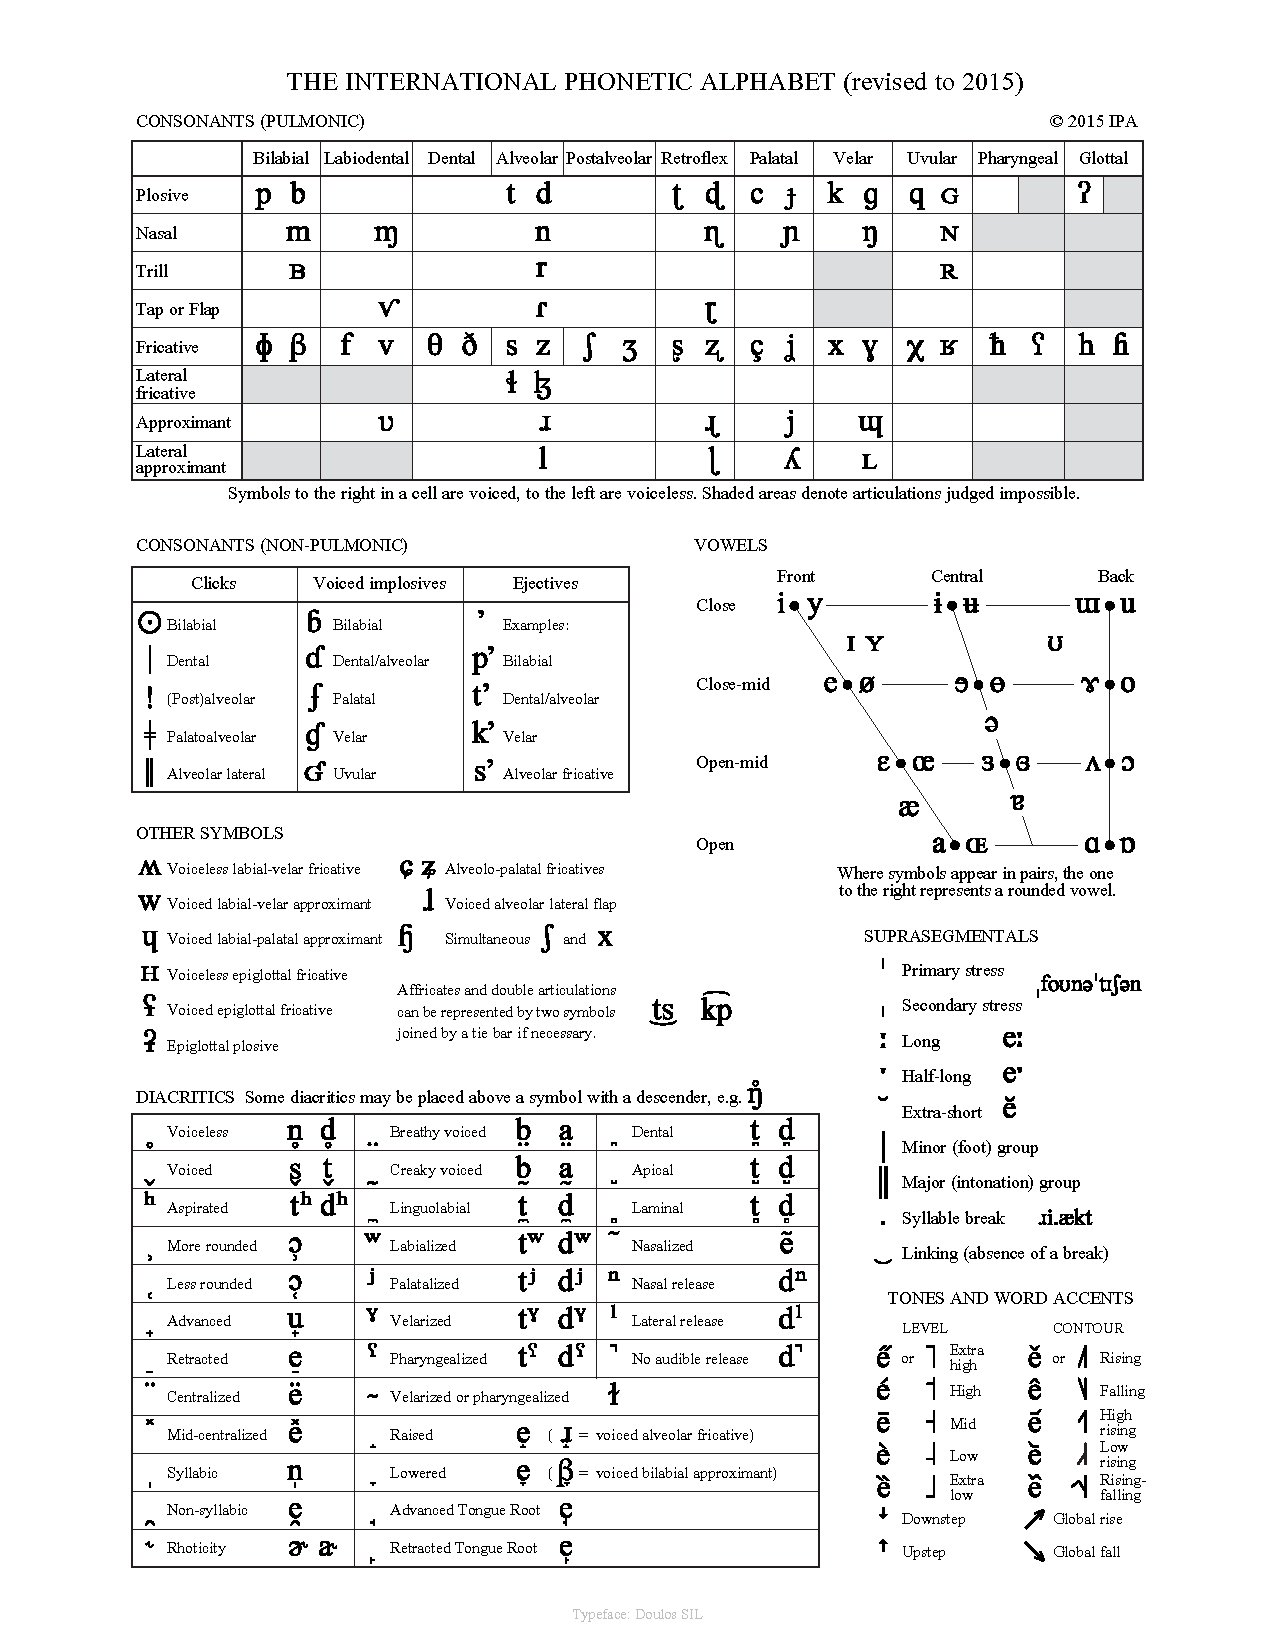
\includegraphics[scale=0.62]{ipaChart}}
    \caption{The International Phonetic Alphabet as defined by the International
    Phonetic Association}
    \label{ipaChart}
  \end{figure}

  \subsection{The Speech Chain}

    The speech chain is a concept that was first popularized by Peter Denes \cite{Denes1993}
    in the eponymous book. The basic concept is that there is a chain of information forming
    an unbroken pathway from the idea that the speaker is trying to convey, to the meaning that
    is interpreted by the listener. In this chain (illustrated in Fig.\ref{speechChain}), information
    is transformed in a number of ways when moving from a speaker's intention to a listener's
    understanding. But, for the purposes of this review, it is important to recognize the
    conceptual contribution of treating speech comprehension as a hierarchical process
    that extracts information from an acoustic signal and passes it up a chain of increasing
    complexity until the content of the message is decoded. In this context, we can then move
    to model the stages of the human speech comprehension system as transformations of
    various types on the fundamental speech input signal.


    One useful example of this kind of modeling is shown in the critical band theory of hearing.
    As sound signals travel through the tympanic membrane and into the inner ear, they
    eventually stimulate the basilar membrane of the cochlea.
    This theory is based on the experimental observation, described further in Section 3.2,
    that the frequency analysis performed
    by the basilar membrane is not uniform. Rather, the membrane is more sensitive
    to some frequencies than it is to others
    \cite{Fastl2007,Rabiner2007}. This varying sensitivity can be described by the equation:
    \begin{equation} \label{eq:1}
      \Delta f_c=25+75[1+1.4(f_c/1000)^2]^{0.69}
    \end{equation}
    $\Delta f_c$ represents the bandwidth associated with a frequency $f_c$ and increases
    as the frequency $f_c$ increases.
    In section \ref{early}, there is further discussion of the physiological
    basis of speech comprehension in
    humans and the various ways in which those processes can be modeled.



    \begin{figure}
      \centering
      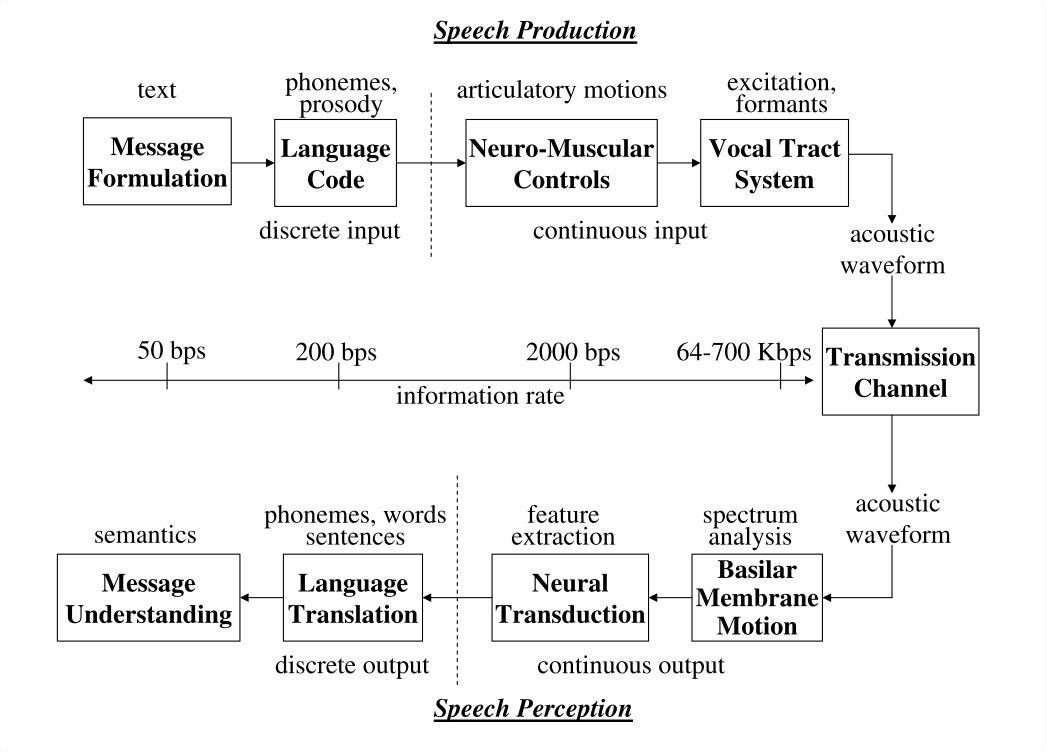
\includegraphics[scale=0.3]{speechChain}
      \caption{The chain of transformations that constitute the `speech chain' as
      described by Denes \cite{Denes1993,Rabiner2007}}
      \label{speechChain}
    \end{figure}

  \subsection{Classes of Phonemes}

    Phonemes can either be classified by their acoustic properties,
    or by the mode of their generation in natural human speech. In the latter
    method, they are typically divided into stops, nasals, fricatives, laterals, rhotics,
    clicks, and vowels \cite{Ladefoged1996}. Though, no language makes use of every speech sound
    that can be produced by the human vocal tract, and some sounds are found much
    more rarely than others. These distinctions are far more useful for the linguistic analysis
    of speech than they are for the acoustic analysis, so we turn to the main acoustic
    differentiation of speech sounds: periodic, voiced speech versus aperiodic, unvoiced speech.
    The difference between these two can be clearly seen from both their waveforms, as well as
    their frequency domain spectra (See Fig.\ref{exampleSpectrogram}).


    \begin{figure}
      \centering
      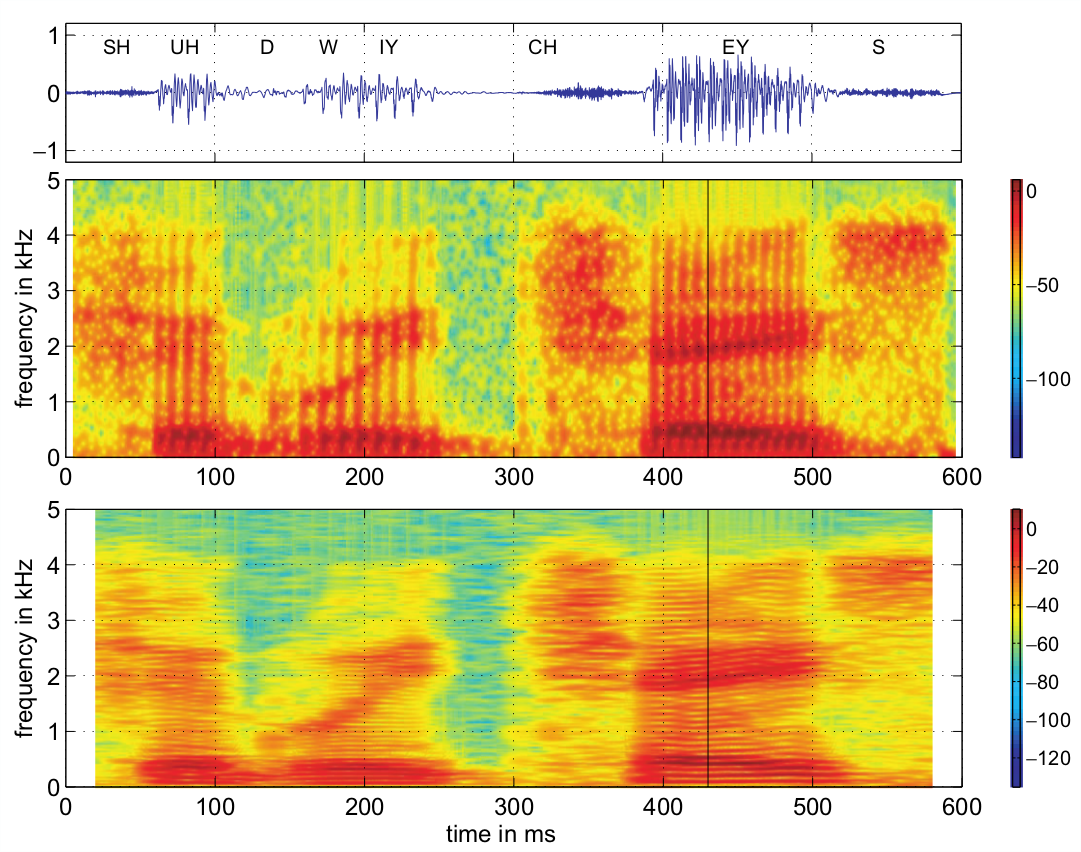
\includegraphics[scale=0.23]{exampleSpectrogram}
      \caption{Waveform and 3D Spectrogram of the phrase `Should we chase' \cite{Rabiner2007}}
      \label{exampleSpectrogram}
    \end{figure}


    The differences between these two classes of speech sounds is explained
    through differences in their modes of production. For instance, the unvoiced
    fricative \textipa{[S]} (the first syllable in Fig.\ref{exampleSpectrogram})
    looks like random noise, while the voiced vowel \textipa{[U]} appears to have
    a definite structure with periodic features. This is because \textipa{[S]} is
    produced by the constriction of airflow out of the mouth through use of the tongue,
    while \textipa{[U]} is produced by the modification of vibrations generated in the
    vocal cords. The fact that voiced sounds are generated by vocal cord vibrations gives
    them a special structure that makes them much easier to identify in the context of
    feature extraction, and makes them important markers in computer speech recognition
    \cite{Gutierrez-Osuna2017}.

    How the brain parses differences between different types of phonemes, particularly
    those that lack discernable spectral content (such as fricatives) is still an area
    of active study. The ability to discern between meaningless noise and a meaningful
    phoneme must rely on information outside of just the spectral content of the
    speech signal itself, as the two might be indistinguishable based on just this information.
    Instead, it is likely that timing and rhythm play an important role in the differentiation
    of speech sounds. The order and precise timing of the delivery of a speech sound has a
    strong effect on how it is perceived and these context effects have strong influences on
    the human perception of speech and language.


    \begin{figure}
      \centering
      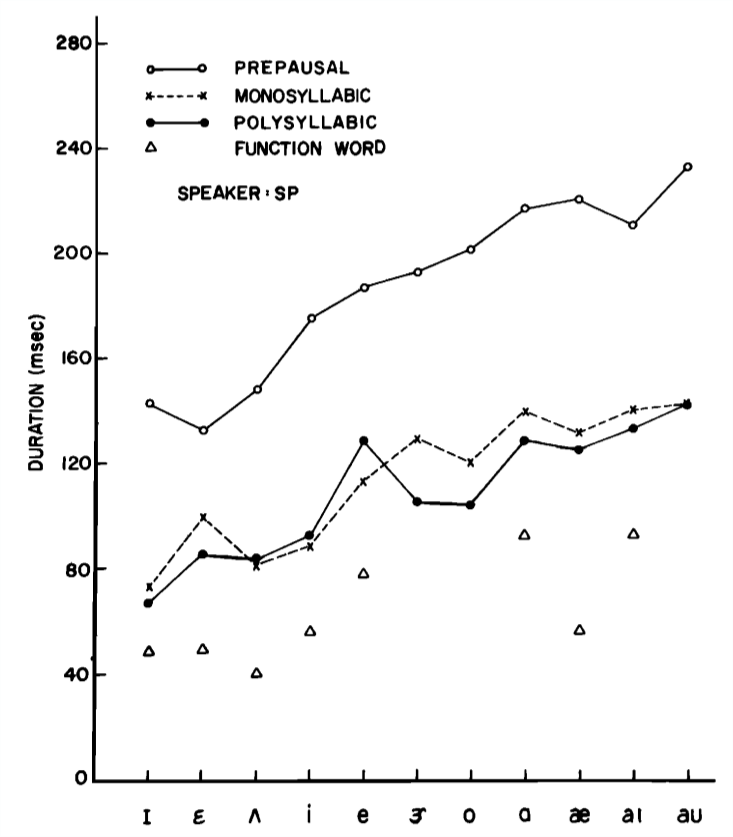
\includegraphics[scale=0.3]{vowelDuration}
      \caption{Average duration of a selection of vowels under three different
      speaking conditions from one speaker \cite{Umeda1975}}
      \label{vowelDuration}
    \end{figure}

  \subsection{Speech Formants}

    An important feature of voiced speech sounds that seems to be critical in their
    recognition are the formants of the vowel sound. Formants are defined as being distinctive
    frequency components of a speech signal that are generated by the resonance
    of the human vocal tract \cite{Denes1993}. They can be seen clearly in the speech spectrogram
    (See Fig. \ref{formants}) as areas of particularly high energy within a certain frequency band.
    Formants come about due to the resonance of the vocal tract. By moving the articulators
    (lips, tongue, etc.), the size and shape of the cavities in the vocal tract are altered and
    therefore so are the resonant frequencies. All vowel sounds are produced through this manipulation
    of the resonant frequencies of the vocal tract which gives them a characteristic, periodic
    structure that can be readily identified.


    By convention, vowel formants are assigned numbers in order of ascending frequency. So, the
    lowest frequency formant of a vowel is assigned $F_1$, the next lowest $F_2$, and so on.
    Many vowels can be distinguished from one another simply by the use of these first
    two formants \cite{Schnupp2011}, making them important markers in both human and computer
    speech recognition. For example, the vowels in Fig.\ref{formants} can be differentiated
    from one another simply by reference to their $F_1$ and $F_2$ frequencies. The importance
    of these formants to biological auditory comprehension was demonstrated in part by
    Young and Sachs (1979) \cite{Young1979}, who showed that auditory nerve discharges in
    response to auditory stimuli reflect the formants when vowels are presented.


    \begin{figure}
      \centering
      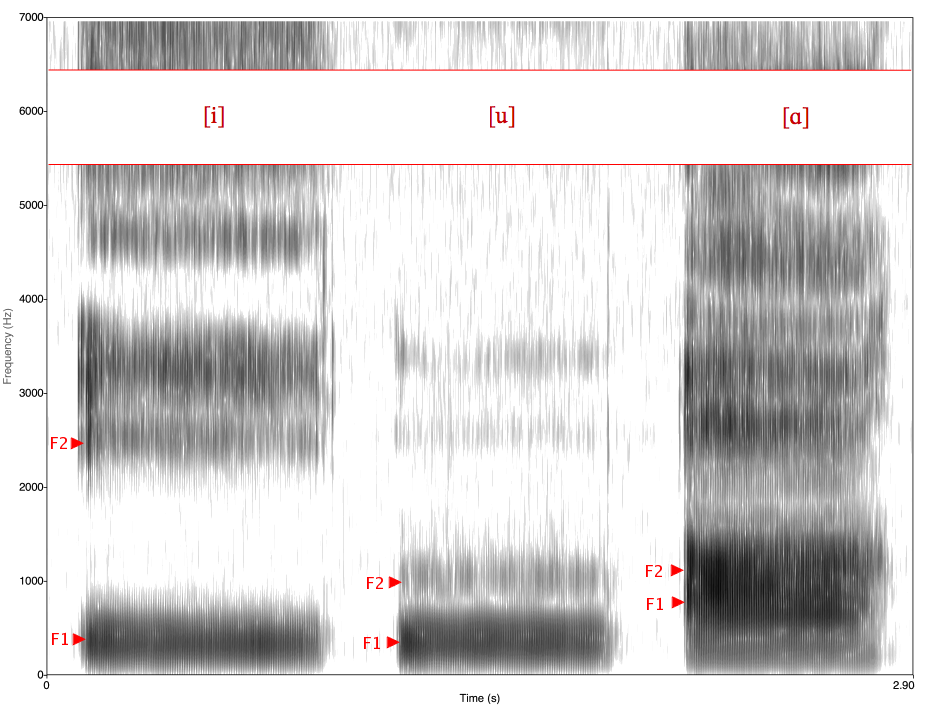
\includegraphics[scale=1.6]{formants}
      \caption{Spectrogram of a native speaker of American English
      pronouncing the vowels \textipa{[i, u, A]} \cite{pict}.}
      \label{formants}
    \end{figure}

  \subsection{Rhythms in Speech} \label{rhythmsInSpeech}

    Fundamentally, speech is rhythmic. It consists of a series of events that have a
    systematic timing and build from smaller components, such as phonemes, into larger
    structures, such as words and sentences, that have their own rhythms as well. The
    cause of this perception of rhythm is the fluctuation of sound intensity over time.
    In the case of speech, modulations less than 16 Hz, with a notable peak at 3-5 Hz,
    are the basis for the syllabic rhythm \cite{Giraud2012,Greenberg2003}.

    One way to characterize these rhythms is through analysis of the modulation spectrum of
    speech. The modulation spectrum is `the spectrum of the temporal envelope of sound and
    reflects how fast sound intensity fluctuates over time' \cite{Ding2017}. In a study of
    a large audio corpus of 9 languages, Ding et al. (2017) \cite{Ding2017} found a remarkably
    consistent peak for the modulation spectrum of spoken language at 2-10 Hz, with a particular
    peak at \textasciitilde 5 Hz. This same 5Hz rate has also been found in empirical studies of syllabic
    rate in a number of languages \cite{Pellegrino2011} and seems to be a consistent, intrinsic
    property of speech, regardless of the language that is being spoken.

    These temporal modulations are likely important to the processing of spoken language in the
    brain as they provide consistent acoustic landmarks for the chunking of incoming acoustic
    signals into discrete units that can then be decoded. The existence of this type of rhythmic
    structure in speech

\section{Early Auditory Processing} \label{early}

  \subsection{The Outer and Middle Ear}

    \begin{figure}
      \centering
      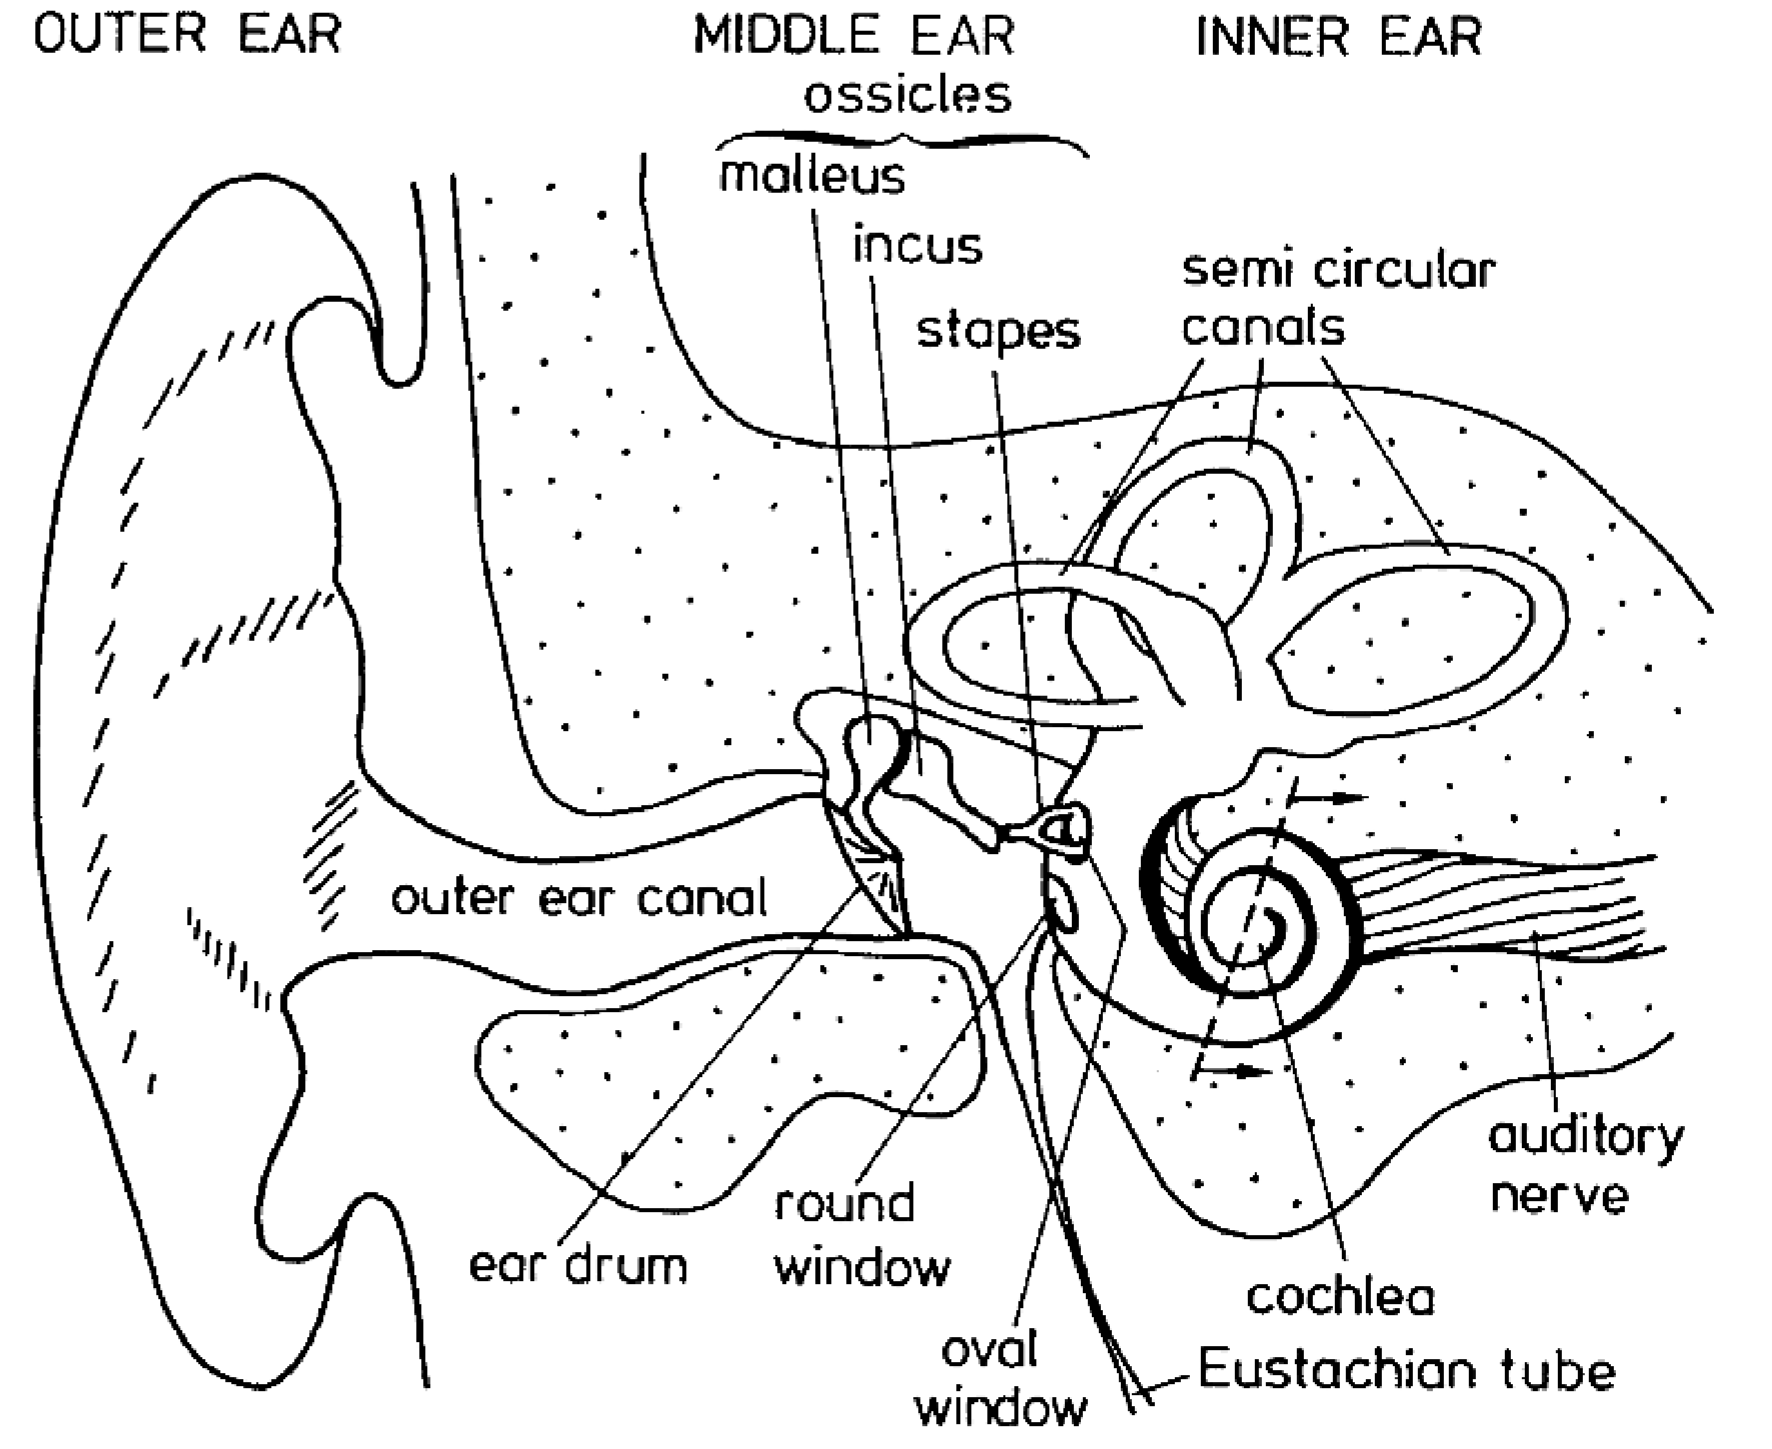
\includegraphics[scale=0.32]{earDiagram}
      \caption{Diagram of the ear from the outer ear to the auditory nerve \cite{Fastl2007}.}
      \label{earDiagram}
    \end{figure}

    Fig.\ref{earDiagram} shows the structure of the human ear and its three sections that
    are responsible for the processing of sound: the outer, middle, and inner ear \cite{Schnupp2011,Rabiner2007}.
    The outer ear, mainly the pinna, functions to redirect sound waves into the ear canal and
    also has an important role related to spatial localization of sounds, particularly in the vertical axis \cite{Kandel2000}.
    The middle ear consists mainly of a series of small bones, known as the ossicles, connected
    to the tympanic membrane towards the outside and to the oval window of the cochlea on
    the inside. These ossicles mainly serve to transform the vibrations in the air into mechanical
    vibrations within themselves via the tympanic membrane. Finally, the inner ear consists of the
    cochlea, which is the one of the most important structures in human hearing. The cochlea is the
    organ that translates the frequency components of an acoustic signal into neural impulses that
    are then transmitted to the brain via the auditory nerve.

  \subsection{The Cochlea and Basilar Membrane}

    The cochlea is one of the most important structures in early auditory processing,
    in that it serves to analyze the spectrum of incoming acoustic signals and then
    conducts that information along the auditory nerve to higher brain areas.
    It does this through a structure known as the basilar membrane, which is a
    membrane that is wound up in the cochlea and serves as the mechanism by which
    vibrations are transduced into neural impulses \cite{Kandel2000}. For the purposes
    of this review, the most important structure in the cochlea is the basilar membrane.

    \begin{figure}
      \centering
      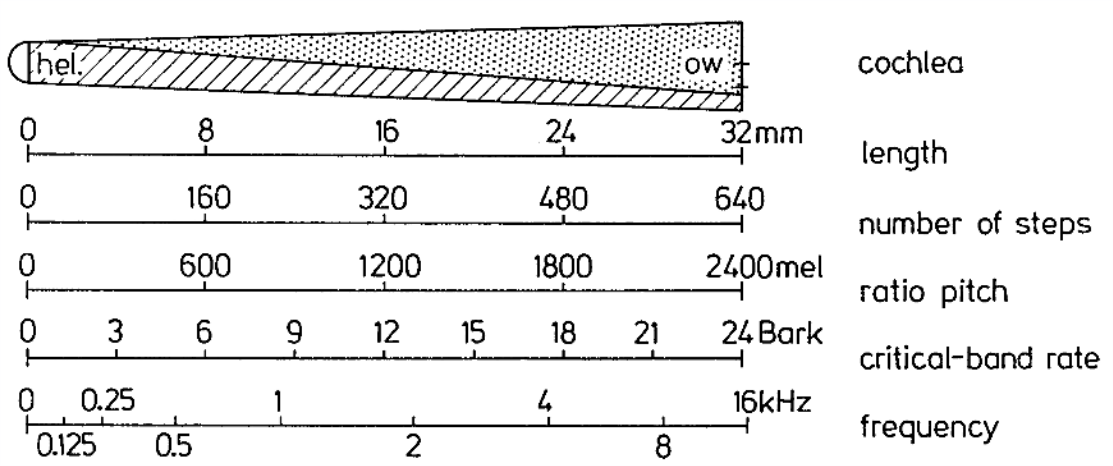
\includegraphics[scale=0.30]{basilarMembrane}
      \caption{Illustration of the unwound cochlea from the helicotrema (left), where low
      frequency sounds are detected, to the oval window (right), where high
      frequency sounds are detected. The number of steps (on the musical
      scale), and the ratio pitch as measured on the mel scale are linear, but the
      frequency response is not.}
      \label{basilarMembrane}
    \end{figure}

    The basilar membrane does this through the mechanical properties that it exhibits.
    It is narrow and stiff at the base of the membrane, where the high frequency sounds
    are detected, becoming more wide and flexible towards the apex of the membrane, the
    site of low frequency sound detection. This divergence in the mechanical properties
    of the membrane along its length allows it to function as a spectral analyzer
    and encode neural representations of the power spectral density of an acoustic signal.
    In essence, the basilar membrane performs
    spectral analysis on complex sounds by being sensitive to different frequencies
    along its length. The mechanical vibrations at these various sites then excite
    the hair cells that are present in those positions, which send neural impulses along
    the fibers that innervate that particular region of the membrane \cite{Kandel2000}.
    The functioning of the basilar membrane also determines the physical limits of
    human hearing in ideal circumstances (without noise, hearing loss, etc.), falling
    at approximately 20 Hz - 20 kHz \cite{Rabiner2007}.

    The intensity of a sound, or frequency band within a complex sound, is encoded
    by the basilar membrane as well. The more intense a sound within a particular
    frequency range, the more intense the vibration and thus the stimulation of the
    hair cells at that point in the membrane. This detection of sound intensity
    is not equal at all frequencies, though. First described by Fletcher and Munson
    and later refined by other researchers, human loudness perception can be modeled
    as a function of frequency (at least in the case of pure tones) \cite{Fastl2007,Fletcher1933,Kandel2000}.
    These curves are still known as Fletcher-Munson curves in honor of the researchers
    that first described them and they compare the intensity of a sound (measured in $dB_{SPL}$)
    with the perceived loudness of that sound (measured in $phon$). As show in Fig. \ref{fletcherMunsonCurve},
    humans are most sensitive to sounds falling within the range of \textasciitilde 2 - 4 kHz and
    are least sensitive to sounds at the lowest ends of the spectrum (\textless 200Hz).

    These findings form the basis for the critical-band theory of human auditory
    perception that is summarized in Eq. \ref{eq:1} in which the basilar membrane
    acts as a bank of band-pass filters that are tuned to be more sensitive
    to some frequencies compared to others.


    \begin{figure}
      \centering
      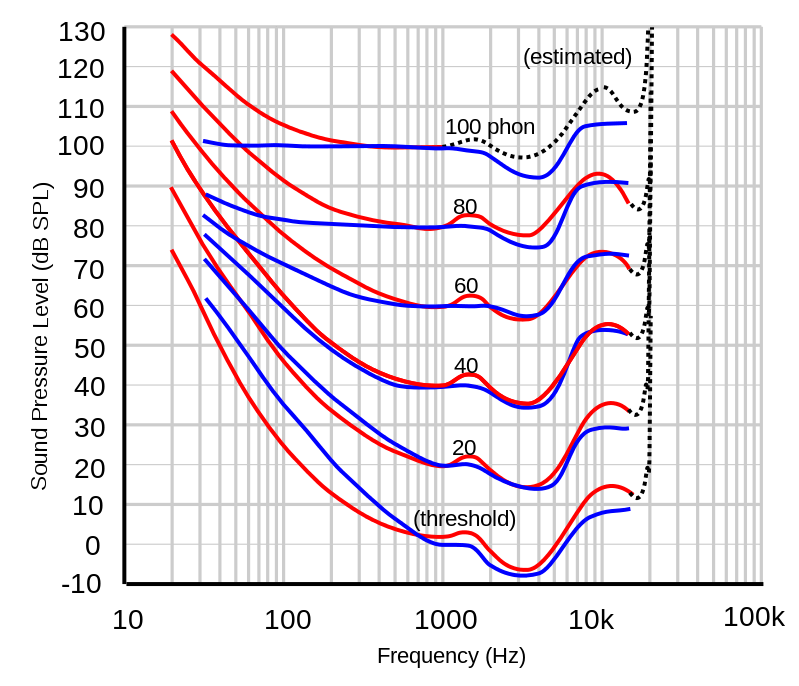
\includegraphics[scale=0.3]{fletcherMunsonCurveWithUnits}
      \caption{Equal-loudness curves in humans. Those defined by the ISO 226:2003 revision
      are show in red and are the accepted standard as of 2014.
      The original Fletcher-Munson curves are shown in blue.}
      \label{fletcherMunsonCurve}
    \end{figure}

  \subsection{Critical Band Theory}

    Understanding this early processing of acoustic signals performed by the
    basilar membrane is crucial to understanding many of the characteristics
    of human auditory perception and therefore speech perception. The varied
    sensitivity of the basilar membrane to signals of different frequencies
    is responsible for both the unequal loudness perception of the human
    auditory system, as well as the nonlinear nature of pitch perception
    illustrated in Fig. \ref{basilarMembrane}. Crucially,
    the responses of these hair cells and the signals that they send along the auditory nerve are the sole
    acoustic inputs that feed into cortical auditory areas and are therefore crucial to understanding
    the processing being done in these higher-level areas. Additionally, this model of cochlear responses to
    acoustic stimuli as a bank of band-pass filters is important in providing temporal information, such
    as the modulation of a frequency modulated (FM) signal, in addition to the spectral information that it
    is tuned for.

    The human auditory system uses the basilar membrane as a mechanical
    means by which to convert an incoming acoustic signal into the frequency
    domain, but does so in a way that is limited by the mechanical properties
    of the membrane itself. This transformation can be accurately modeled using a
    technique known as mel-frequency cepstrum coefficient (MFCC) analysis \cite{Davis1980,Noll1967}.

\section{Cortical Auditory Processing} \label{corticalAuditoryProcessing}

  In the above sections, the emphasis has been on the properties of the
  acoustic stimulus itself, its important features, and the mechanisms by
  which it is detected by the human auditory system. This chapter is dedicated
  to the transformation and integration of that acoustic information after it
  has been detected by the auditory system. Once an acoustic stimulus has
  been transformed into neural impulses by the machinery of the inner and outer
  ear, it proceeds through the brainstem and into the cortex. Roughly,
  information travels from the cochlea to the cochlear nuclei of the brainstem,
  the superior olive, the inferior colliculus, the medial geniculate nucleus of
  the thalamus, and finally to the primary auditory cortex
  \cite{Hickok2007,Webster1992}. This outline of the auditory pathway is
  clearly a large oversimplification. Brainstem and subcortical innervation
  sites are more numerous than described above, and there are also significant
  efferent connections from the higher auditory processing areas all the way
  down to the cochlear neurons themselves \cite{Kandel2000,Webster1992}. This
  overview is meant to provide a rough sketch to demonstrate the hierarchical
  and interconnected nature of the auditory processing pathways as well as to
  give a general view of how information proceeds from the ear to the cortex.


  This pathway shares some features of the visual processing pathway. It is
  hierarchical, but not strictly so, and it contains significant
  back-projections and divergent pathways \cite{Webster1992,Hickok2007}.
  Hickok and Poeppel, two prominent voices in the field, maintain that there
  are actually two parallel cortical pathways for acoustic information much
  like the parallel processing pathways found in the visual system
  \cite{Hickok2007,Hickok2004,Hickok2000}. The ventral auditory processing
  stream is thought to underlie the conversion from acoustic signals into
  lexical and semantic representations. The analogy could be drawn to the
  ventral visual stream, which is thought to mainly be responsible for visual
  object recognition. In a similar way, the ventral auditory stream underlies
  the ability to recognize acoustic `objects' and connect those to phonological
  or semantic meanings \cite{Parker2005,Rauschecker2009}. The dorsal stream of
  the auditory pathway has a less well-understood function, but it is thought
  to be involved in sensorimotor integration in much the same way as the dorsal
  visual stream is. In particular, Hickok and Poeppel theorize that this
  network is crucial in the development of speech as it integrates the sounds
  that are perceived and facilitates the motor learning task of learning to
  speak.

  A competing theory put forward by Angela Friederici \cite{Friederici2011} is
  that there are actually two ventral pathways and two parallel dorsal pathways.
  In this theory, there is one ventral pathway from roughly Broadmann's area 45
  to the temporal cortex and another from the frontal operculum (FOP) to the
  uncinate fascile (UF). These two ventral pathways are hypothesized to mainly
  be responsible for language processing and the processing of adjacent elements
  in an audio signal. The two dorsal pathways are thought to connect from the
  temporal cortex to the premotor cortex, as well as from the temporal cortex
  to Broadmann's area 44. The first pathway is thought to mainly support
  auditory motor functions similar to those proposed by Hickok and Poeppel,
  while the second is thought to be involved in more high-level language
  processing functions. Specifically, the second pathway is thought to provide
  a complement to the ventral streams in that it connects information that
  is not adjacent in the auditory stream and allows for grammatical analysis
  and connections.

  \subsection{Primary Auditory Cortex} \label{primaryAuditoryCortex}

    \begin{figure}
      \centering
      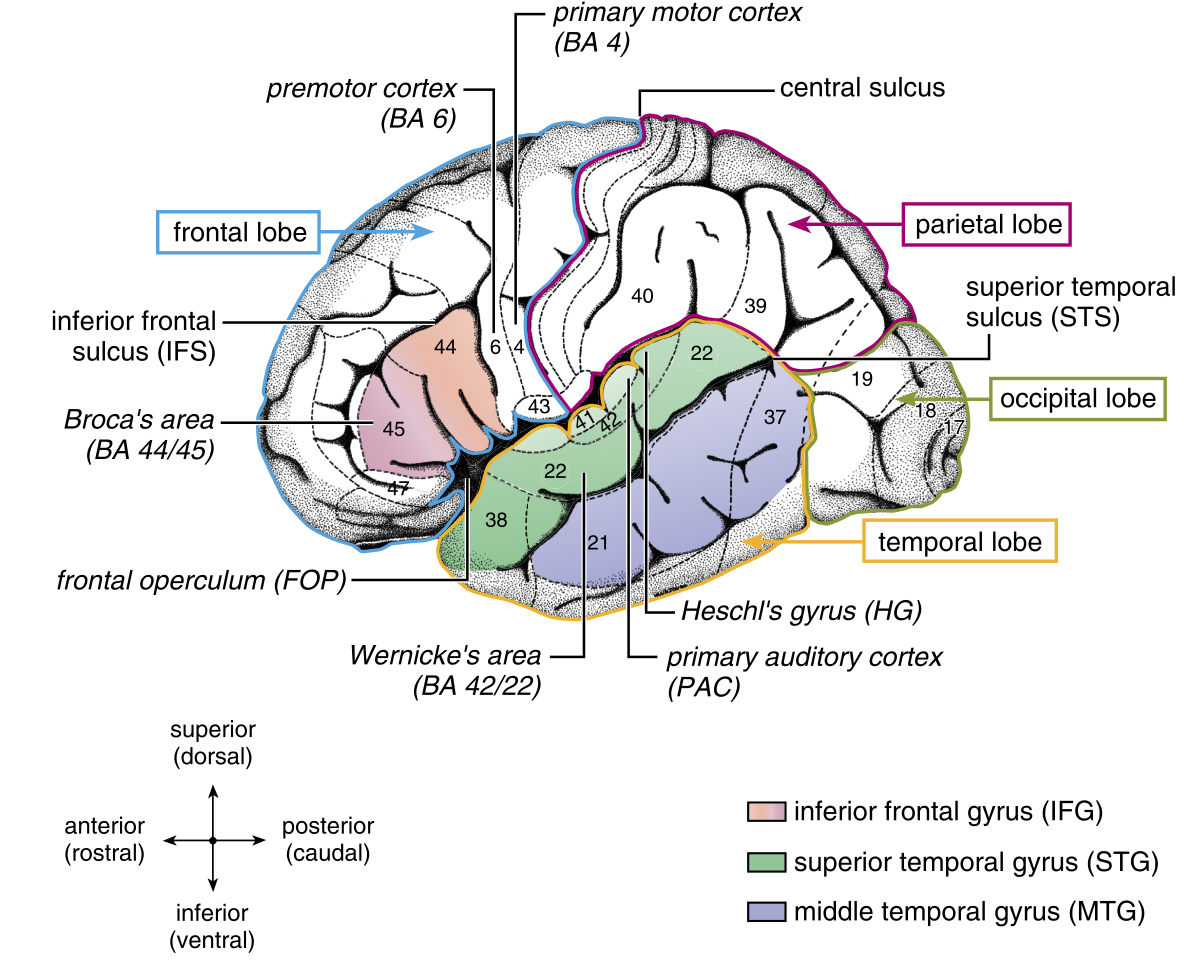
\includegraphics[scale=0.25]{primaryAuditoryAnatomy}
      \caption{This figure shows the gross anatomy of the left hemisphere
      of the human brain. The lobes, Brodmann's areas, and other areas
      of interest have been highlighted. \cite{Friederici2011}}
      \label{primaryAuditoryAnatomy}
    \end{figure}

    The primary auditory cortex (A1) is the main target of auditory information
    from the sensory neurons in the cochlea and is the backbone of auditory
    perception. It is located on the superior temporal gyrus
    (see Fig. \ref{primaryAuditoryAnatomy}) and can be divided into a primary
    area and various belt or peripheral areas \cite{Purves2001}. A1 is organized
    tonotopically, meaning that there is a separation by frequency of the
    incoming auditory signals, and that neighboring neurons respond to
    neighboring frequencies \cite{Lauter1985}. Organization of A1 is analogous
    to the topographical mapping that can be found in V1, and mirrors the
    tonotopic organization of the basilar membrane, discussed above.
    Therefore, A1 can be said to
    have a frequency `axis', groupings of neurons that react selectively to the
    frequency content of incoming auditory signals. Additionally, A1 contains an
    orthogonal `axis' that processes information related to the binaural aspects
    of incoming auditory signals and may serve localization or source
    identification purposes \cite{Purves2001}.


    Bilateral destruction of A1 results in cortical deafness, resulting in a
    total loss of hearing faculties in those affected. In order to manifest,
    this disorder requires total bilateral destruction of A1. Due to this, as
    well as the relatively high degree of redundancy in subcortical auditory
    structures, the disorder is quite rare \cite{Polster1998}. Additionally,
    subcortical processing of auditory signals may preserve some auditory
    capacities even in patients with this condition \cite{Cavinato2012}. More
    commonly, following damage to the cortical auditory areas are the conditions
    of auditory agnosia, pure word deafness, and phonoagnosia.

    Auditory agnosia
    is a condition in which patients are incapable of identifying sounds such
    as coughing or whistling, but show no evidence of impaired auditory speech
    comprehension. Pure word deafness is essentially the opposite of auditory
    agnosia, where patients are incapable of comprehending speech while
    maintaining their ability to speak, read, and identify sounds.
    Interestingly, some patients with pure word deafness retain their ability
    to extract information about a speaker (such as age, sex, etc.) based on
    their speech \cite{Polster1998}. Phonoagnosia is a condition analogous to
    prosopagnosia (inability to recognize familiar faces), where patients
    lack the ability to recognize familiar voices.


    These conditions provide insights into the different functions that are
    performed by the auditory processing system and demonstrate that these
    functions can be dissociated without disrupting the system completely. This
    observation points to the fact that the human auditory system is attempting
    to extract multiple types of information from an incoming auditory signal
    and that the methods for extracting this information involve separate
    cortical processing mechanisms.

  \subsection{Broca, Wernicke, and Heschl}

    In the following section, I will review three brain areas critical to
    speech perception outside of A1. These are Heschl's gyrus, Wernicke's 
    area, and Broca's area. Each of these brain regions form part of the network
    that is responsible for speech perception and play distinct, but
    interrelated, roles in the perception of spoken langauge.

    [section on Heschl]

    Central to any analysis of speech perception is Heschl's Gyrus (HG). Named 
    in honor of the Austrian anatomist Richard Heschl, who is considered the
    first to describe transverse temporal gyrus, this area is critical to all
    auditory perception, including speech perception. HG is located in the 
    lateral sulcus, primarily consisting of Brodmann's areas 41 \& 42.

    The exact location and organization of HG differs between individuals, with 
    some having having an HG that is split by a sulcus, or some even having 
    full duplications of the gyrus located posteriorly to 
    the typical location \cite{citationNeeded}.
    This complication is to be expected, as language and auditory areas often 
    have individual variations in their exact locations and can often be 
    difficult to locate on a single individual. 

    Even with this difficulty, the structural and functional aspects of HG 
    have become clear over years of experimentation in both humans 
    and non-human animals. The primary auditory cortex is located partially 
    within HG, though some areas of A1 are not located within HG and it does 
    not take up the entirety of the gyrus.


    [section on Wernicke]

    Broca's area has been a well known area of language processing since
    Pierre Paul Broca, in 1861, described two patients that had lost the
    ability to speak following damage to the inferior frontal gyrus
    \cite{Dronkers2007}. The condition resulting from damage to this area,
    characterized by problems with fluency in speaking and difficulty with
    complex grammar, is called Broca's aphasia. Today, Broca's area is also
    defined by the Brodmann areas 44 and 45, or the pars opercularis and pars
    triangularis, and continues to be a heavily studied area of the brain.

    Broca's area has been historically associated with speech
    production through numerous lesion studies and case studies of aphasic
    patients \cite{Dronkers2007}. It was also found to have significant
    connections both to motor control areas, such as the premotor cortex,
    as well as to other language areas, such as Wernicke's area, through the
    arcuate fasciculus and other pathways \cite{Friederici2011}. These findings
    further reinforced the idea of Broca's area as, primarily, a facilitator of
    sound-to-motor mappings. Though it was originally believed that Broca's
    area was mainly involved in
    speech production rather than comprehension, more recent evidence suggests
    that it is involved in speech comprehension as well. In
    particular, evidence from PET and fMRI studies points to the role of Broca's
    area in the processing of syntactically complex or semantically ambiguous
    sentences \cite{Rodd2005,Ojanen2005,Zurif1980}. Some studies have found
    evidence that this area is also involved in more low-level phonetic or
    semantic processes \cite{Zatorre1992}, though this remains controversial
    and the subject of ongoing debate \cite{Hickok2013,Friederici2011}. Though
    there is evidence that BA 44 \& 45 play a role in speech comprehension, there
    is also significant evidence from Wada procedures and congenitally anarthric
    patients that the loss of motor speech production capacities does not
    preclude the ability to comprehend speech \cite{Hickok2013}.


  \subsection{Speech Comprehension vs. Speech Production}

    There is ongoing debate about the involvement of speech production
    circuits in speech comprehension. There are multiple competing theories
    about this. Some claim that speech production circuits, through
    mirror neuron type mechanisms, are essential for speech comprehension
    to function properly. Others claim that speech production circuits are not
    necessary at all for the proper functioning of speech comprehension.

\section{Entrainment} \label{entrainment}

  \subsection{Brainstem Entrainment} \label{brainstemEntrainment}

    The Auditory Brainstem Response (ABR) is a well-known neural response to
    auditory stimuli that was discovered more than 40 years ago
    \cite{Jewett1971,Jewett1970} and has seen widespread use in clinical
    settings for determining auditory thresholds or diagnosing neuropathologies
    \cite{Skoe2010} and is especially popular for hearing screening in infants.
    Measurement of this response is one of the most common clinical applications
    of auditory evoked potentials and the typical waveform is well
    characterized.

    The test typically consists of presenting a subject with a series of click
    stimuli while recording neural activity through surface electrodes placed on
    the scalp. The averaged activity is then examined for the characteristic
    response that develops over a window of \textasciitilde 10ms and consists
    of a series of waveform peaks labeled \textit{I-VII}
    \cite{Sininger1993,Bhattacharyya2017}. This activity is a stimulus-driven
    response that is generated in the brainstem and the auditory nerve and as
    such cannot be equated with the conscious perception of a stimulus, but
    does seem to be highly predictive of a subject's level of hearing loss
    \cite{Sininger1993}.

    More recently, there has been work involving the measurement of the ABR in
    response to complex stimuli, as opposed to the simple clicks or tones that
    were used previously. For example, Galbraith et al. (1995)
    \cite{Galbraith1995} found that intelligible speech could be recovered from
    the ABR that is recorded while the subject is presented with speech stimuli.
    Further studies have been conducted looking at a diverse range of stimuli
    including words and phrases, music,

  \subsection{Cortical Entrainment} \label{corticalEntrainment}

    In addition to entrainment occurring in the brainstem, it is also possible
    to measure cortical entrainment in response to acoustic stimuli with methods
    such as electroencephalography and magnetoencephalography. This type of
    entrainment typically has the best correspondence to the temporal
    modulation of the speech signal
    \cite{Ding2014a,Ding2014,Nourski2009,Horton2014}, including both amplitude
    envelope modulation and frequency modulation. This cortical entrainment
    seems to be linked to a number of behavioral factors, such as attention
    \cite{Dmochowski2016,ZionGolumbic2013} as well as engagement with the
    stimulus \cite{Dmochowski2017}. This entrainment is clearly an exogenous
    stimulus-driven process, which is illustrated by the consistent responses
    elicited across subjects by the same audio or visual stimuli
    \cite{Cohen2017,Petroni2017}.

    Interestingly, speech remains intelligible despite a large amount of
    information in the speech signal being destroyed. Speech information is
    resistant to both degradation of temporal as well as spectral information
    \cite{Silipo1999,Drullman1994}. Barring total elimination of temporal and
    spectral information, it is only when both are sufficiently degraded that
    speech becomes unintelligible \cite{Elliott2009}. Related to this, the
    phenomenon of speaker gender identification is also reliant on similar
    information and can be modulated by changing the information present in the
    temporal and the spectral domain. Elliott and Theunissen \cite{Elliott2009}
    found that speaker gender identification rate can be significantly
    degraded by removing spectral modulations between 3 and 7 cyc/Hz and that
    this specifically reduced the subjects' ability to correctly identify
    female speakers. They postulated that this is because the female vocal
    spectrum has more power in this specific range and this is what
    contributes to `sounding like' a female speaker. Clearly, there is more
    information than just that necessary for comprehension that is embedded
    in the temporal and spectral modulations of speech and it is important to
    parse out what is necessary for the comprehension of speech and what
    information is supplemental, but not necessary to the bare comprehension
    of speech.

  \subsection{Innate Brain Rhythms} \label{innateBrainRhythms}

    There exist a number of neural rhythms that are innately present in the
    human brain. Roughly speaking, these are divided into $\alpha$ (8 - 12 Hz),
    $\beta$ (12 - 30 Hz), $\theta$ (4 - 8 Hz), $\delta$ (1 - 4 Hz), $\gamma$
    (30 - 80 Hz), and high $\gamma$ (80 - 150 Hz)
    \cite{Muresan2008,Rangaswamy2002}. These are roughly divided by the
    frequency of the oscillations and their suspected behavioral correlates.
    There is clearly overlap between these categorizations and it is difficult
    to make very clear distinctions between the various classes of neural
    oscillations. Despite this, there are some clear behavioral correlates in
    each of these frequency bands, and there have been attempts to localize the
    neural circuits responsible for their generation \cite{Michel1992}.

    Some of these rhythms are particularly relevant for the study of speech
    processing as they appear to have the same frequency as the typical speech
    rhythm and their power in EEG signals increases as a function of
    intelligibility. Particularly important to speech processing appear to be
    the $\delta$, $\gamma$, and $\theta$ rhythms \cite{Ghitza2009,Meyer2018}.
    In the case of the $\theta$ rhythm, Oded Ghitza has been a particularly
    strong advocate for the idea that the $\theta$ rhythm is crucial to parsing
    the speech signal into syllabic chunks which are the fundamental unit of
    speech processing. He refers to this fundamental unit as the
    `theta-syllable' \cite{Ghitza2013a} and claims that it is central to the
    theory of speech comprehension as a faculty facilitated by cortical
    entrainment to speech signals. In this view, the theta-syllable is defined
    as `a theta-cycle long speech segment located between two successive vocalic
    nuclei'. A vocalic nucleus is the critical section of a syllable (often a
    vowel) that can be preceeded or followed by other marginal sounds (often
    consonants). For example, the word \textit{window} can be divided into the
    syllables \textipa{/"wIn/} and \textipa{/doU/}. In the \textipa{/"wIn/}
    syllable, the \textipa{/I/} sound functions as the nucleus while the
    \textipa{/w/} and \textipa{/n/} sounds are on the margins of that nucleus.

    In this interpretation, the theta rhythm is essentially the `master' rhythm
    that is responsible for the main chunking of the incoming speech stimulus
    and leads to the efficient parsing of syllables. This is crucial to
    understanding speech comprehension because of one of the most important
    mysteries in this area is how the brain chubnks information into syllables
    that can then be parsed and transformed into higher-order representations.
    Without the ability to transform incoming acoustic information into smaller
    `chunks', the brain would have no ability to separate out syllabic
    information and parse what the speech information in a given chunk of time
    is. Instead, it would appear more as an undifferentiated mass.

  \subsection{Phase Entrainment}

    It has been demonstrated that cortical neurons entrain their phase to the
    oscillations present in speech stimuli, but the causal mechanism of this
    entrainment is still being debated in the field. Some claim that it is
    caused by entrainment to low-level features of speech sounds, basically a
    version of an auditory steady-state potential (such as those found in the
    brainstem discussed in section \ref{brainstemEntrainment}). Other
    researchers maintain that this phase entrainment is a product of more
    high-level speech sound features and reflects a processing of information
    carried in the speech signal by the brain.

    Zoefel and VanRullen \cite{Zoefel2016} address this question by presenting
    subjects with mixed speech/noise stimuli that retain the patterns of
    higher-level features, but do not have the fluctuations in spectral content
    and sound amplitude that some claim is the basis for the phase entrainment
    response. They found that neural phase entrainment occurs despite the
    missing low-level content, indicating that it is the higher-level features
    that drive this response. Additionally, they find that reversing their
    speech/noise mixture stimuli does not eliminate the phase entrainment
    response. This finding seems to indicate that the entrainment is in
    response to higher-level features, but only those that are acoustic in
    nature and not linguistic features, as those are absent in time-reversed
    speech.

    What, exactly, the functional role of this entrainment to the speech
    envelope is remains a topic of debate in the field, but there has recently
    been strong evidence to support the hypothesis that cortical entrainment to
    the speech envelope facilitates comprehension of the speech signal
    \cite{Ding2014a,Ding2012,OSullivan2015}.


    This hypothesis is supported by evidence correlating behavioral measures of
    comprehension of a speech segment to the level of neural envelope-following
    response that is found. These experiments, though, simply show that neural
    entrainment and speech comprehension co-occur. On their own, they fail to
    make the causal connection between neural entrainment and comprehension.

    These envelope-following responses found in response to acoustic stimuli
    differ from the

  \subsection{Envelope Following and Brain Rhythms}

    The fact that cortical neurons track the amplitude envelope of speech
    signals is now well-known and is considered an important part of the speech
    processing pathway. But, the interaction between natural cortical rhythms
    (discussed in Section \ref{innateBrainRhythms}) and the envelope following
    response is still not completely understood, and its functional role remains
     a subject of debate. There is abundant evidence that broad-spectrum EEG
     signals can be used to decode which speaker is being attended to by a
     subject in a cocktail party scenario \cite{Horton2014,DeTaillez2018}, but
     these studies only offer a partial picture of the role of cortical
     envelope-following responses in speech comprehension.

    For instance, Zion Golumbic et al. \cite{ZionGolumbic2013} were able to
    localize the envelope tracking response both in terms of cortical location
    as well as which frequency band was recruited for entrainment using
    electrocorticography (ECoG) in a cocktail party scenario with two speakers.
    They found found that there is a significant ability to predict which
    speaker is being attended in two different frequency bands that they term
    `low-frequency' (1-7 Hz) and `high gamma' (70-150 Hz). Further, they found
    that cortical locations in which these two frequency bands possessed
    significant predictive power differed. Both showed a very strong response
    in the superior temporal gyrus, which is to be expected given that is the
    location of the early cortical auditory areas, but the high gamma band
    showed a more widespread distribution around the brain, while the
    low-frequency band was more concentrated in frontal and temporal areas.

    These findings point to the conclusion that the envelope following response
    is not monolithic, and that there are multiple functional roles filled by
    the envelope following response.

    One of the most popular theories currently is that speech signals are
    essentially a quasi-rhythmic input which certain innate cortical rhythms are
    recruited to track. This tracking then enables both the exclusion of
    irrelevant speech signals \cite{Horton2014,OSullivan2015} as well as the
    syllabic parsing that is thought to be accomplished by the innate theta
    oscillations in the cortex \cite{Doelling2014,Ghitza2013b}.

    This brings up a large controversy in this field of study, which is the
    question of whether neural entrainment occurs because of the recruitment of
    natural neural rhythms that are simply used for alignment and parsing of the
    incoming speech signal, or whether these oscillations are actually
    generated by the speech signal itself and do not rely on oscillatory
    activity that is always ongoing in the cortex. This distinction is
    important because it colors how the increase in stimulus-aligned activity
    is interpreted. In the case of innate, ongoing oscillations being recruited
    to speech comprehension purposes, the activity that is elicited by
    presentation of a stimulus is used in `chunking' the incoming speech signal
    into segments that can be processed for lexical information and then
    combined to give some type of semantic meaning to a sentance. On the other
    hand, if the increase in stimulus-aligned activity is due to the
    emergence of a signal in the brain that tracks the amplitude envelope of
    the incoming speech signal, then it would seem that the analysis being
    performed in the brain is not of the `chunking' type, but involves
    synchronizing to the rate of the incoming speech signal and using
    information other than the relation of the incoming speech signal to
    innate oscillatory activity to process and comprehend speech.

  \subsection{Effects of Visual Information on Entrainment}

    Though this review is focused on the processing of auditory information, it
    is worth taking time to discuss the contributions of other modalities to
    the auditory comprehension process and how those other modalities might
    influence the neural signals that we can measure. Auditory information,
    especially in the case of speech, is rarely present without any visual
    input. When we are speaking with another individual, that person's facial
    expressions, lip movements, and body language all influence the our
    understanding of their speech. Especially in the case of speech that is
    difficult to hear or ambiguous, visual cues provide significant information
    that guides the comprehension of the auditory signal.

    For instance, it is well documented that, especially under noisy
    conditions, being able to see a speaker's face contributes significantly to
    the ability to understand that speaker \cite{Sumby1954,Erber1969}.

  \subsection{Comprehension Effects of Entrainment}

    In recent years, there has been a growing body of literature that supports
    the hypothesis that cortical entrainment to the temporal modulation of
    speech is the critical process that enables speech comprehension
    \cite{Meyer2018,Morillon2015,ZionGolumbic2013,Doelling2014}. This
    entrainment is found in both frequency (FM) and amplitude (AM) modulation,
    though the two are not independent \cite{Ding2009}. Ding \& Simon (2009)
    \cite{Ding2009} find that for a signal that is both frequency
    ($f_{FM}=40Hz$) and amplitude ($f_{AM}\leq 15Hz$) modulated, there is an
    auditory steady-state response at both $f_{FM}$ as well as at $f_{AM}$ but
    that the response at $f_{FM}$ is amplitude and frequency modulated with
    fundamental frequency $f_{AM}$. This points to the fact that when we speak
    about entrainment of signals in the brain there are multiple different
    `sites' of entrainment and that neural oscillations can be entrained to
    multiple features of a stimulus.

\section{Connecting Sounds with Meanings} \label{meaning}

  Up to this chapter the discussion in this paper has mainly focused around the
  transduction of incoming acoustic speech signals into some type of neural
  representation. This computation serves as the basis for speech comprehension
  and any complete account of the human ability to understand complex
  hierarchical speech is incomplete without it. Now I will turn to a very brief
  account of the next stage of the language comprehension process, which is
  the connection of these neural representations of incoming speech signals
  with internal lexical and semantic representations that ultimately give rise
  to the \textit{understanding} of speech, rather than the mere
  \textit{representation} of speech.

\newpage
% \nocite{*}
\printbibliography

\end{document}
